\chapter{引言}\label{chap:introduction}
%当前,一颗GPU芯片上集成的核心数越来越多,GPU体系结构也在非常快速的演变。目前主要的高端GPU芯片厂商有NVIDIA和AMD。主流的GPUs架构有NVIDIA Kepler,Maxwell,Pascal和Volta GPU;AMD Fiji,Vega10,Vega20 GPU。由于每一代的GPU架构都会发生变化,我们就需要在新的架构上重新做优化工作。不幸的是,我们没有可用的性能上界分析方法和工具。在实际中,开发人员通过算法的分析和积累的经验,采用多种优化手段来编写高效的kernel。Kernel编写人员可能会通过性能分析工具(如NVVP\citepns{profiler2011nvidia})的分析结果来指导进一步的优化。然而,这样并不能知道现在优化的结果距离性能上界还有多远。
%
%对于AMD GPU,其官方并没有提供良好的性能分析工具。本文通过手工汇编优化的手法,在Fiji 和Vega GPU上实现的矩阵乘性能达到95\%。
%矩阵乘是BLAS Level3的标准子程序,是科学计算中的核心数学计算。提高矩阵乘的性能对加速BLAS数学库具有重要意义。
%
%本章首先阐述多核处理器的发展历程,从中引出GPU并行体系结构,讨论GPU并行程序设计的方法,然后阐明本文的研究动机,列出本文的主要贡献和组织结构。

随着摩尔定律的即将终结,后摩尔时代计算机体系结构的发展成为了人们关注的重点。当前的数据在经历着爆炸式增长,传统的CPU已经无法满足实际应用场景对计算性能的极致追求。当前处理器主频已经接近上限,无法简单地通过提高主频来获得计算性能的提升,处理器设计朝着多核、众核的方向发展。GPU便是一种众核并行处理器。

当前,一颗GPU芯片上集成的核心数越来越多,GPU体系结构也在非常快速的演变。目前主要的高端GPU芯片厂商有NVIDIA和AMD。主流的GPUs架构有NVIDIA Maxwell,Pascal和Volta GPU;AMD Fiji,Vega GPU。由于每一代的GPU架构都会发生变化,编程人员就需要在新的架构上重新做优化工作。不幸的是,我们没有可用的性能上界分析方法和工具。在实际中,开发人员通过算法的分析和积累的经验,采用多种优化手段来编写高效的kernel。Kernel编写人员可能会通过性能分析工具(如NVVP\citepns{profiler2011nvidia})的分析结果来指导进一步的优化。然而,这样并不能知道现在优化的结果距离性能上界还有多远。

对于AMD GPU,其官方并没有提供良好的性能分析工具。本文通过手工汇编优化的手法,在Fiji 和Vega GPU上实现的矩阵乘效率达到95\%。矩阵乘是BLAS Level3的标准子程序,是科学计算中的核心数学计算。提高矩阵乘的性能对加速BLAS数学库具有重要意义。

本章首先阐述多核处理器的发展历程,从中引出GPU并行体系结构,讨论GPU并行程序设计的方法,然后阐明本文的研究动机,列出本文的主要贡献和组织结构。

\section{通用并行处理器概述}

通用并行处理器(GPGPU General Purpose Graphic Processing Units)是近些年提出的概念,通用并行处理器从图形处理(GPU Graphic Processing Units)发展而来。早期的图形处理器只为图形和游戏的渲染而设计,最早进入该领域的厂商有NVIDIA和ATI。AMD为了增强其图形处理器的设计能力,在2006年以54亿美元收购ATI,成为一家同时具有CPU和GPU研发能力的芯片公司。之后,随着并行计算的需求越来越多,GPU也设计出符合这种趋势的SIMD或SIMT架构。NVIDIA和AMD分别采用CUDA(Compute Unified Device Architecture)和OpenCL这两种编程模型来简化并行程序设计的复杂度。自此,GPU不仅用于图形和游戏渲染,而且也可用于通用并行计算。GPU正往GPGPU方向发展。

现代GPU在产品线上,分为两种,一种是图形处理卡,另一种是计算卡。其中计算卡没有图形输出接口,在设计上去掉了用于图形渲染的相关部件。NVIDIA GPU在产品线上分为Geforce系列和Tesla系列。Geforce GPU既可用于图形渲染也可用于通用并行计算。Tesla系列只能用于通用并行计算,同时Tesla计算卡要比Geforce图形卡价格高很多。AMD GPU在产品线上有Vega56,Vega64系列图形卡和INSTINCT系列计算卡。当前NVIDIA占据着绝大部分GPU市场,具有垄断地位。在前几个月,NVIDIA刚刚公布的用户手册中,就宣布禁止在数据中心使用Geforce系列显卡,使得数据中心的建设成本极大增高。随着大数据,深度学习的兴起,传统CPU计算已经无法满足现有应用对计算的需求,GPGPU应运而生。大数据应用对处理器吞吐量要求很高,而GPGPU是一种面向通量计算的可编程加速器,非常适用于现有的应用。通用并行计算也从只做传统的科学计算,到现在的将通用并行计算技术用于大数据和深度学习领域。NVIDIA GPU架构历经了Tesla,Fermi,Kepler,Maxwell,Pascal和Volta架构的演变(如图\ref{fig:nvidia_gpu_roadmap})。

\begin{figure}[!htbp]
	\centering
	%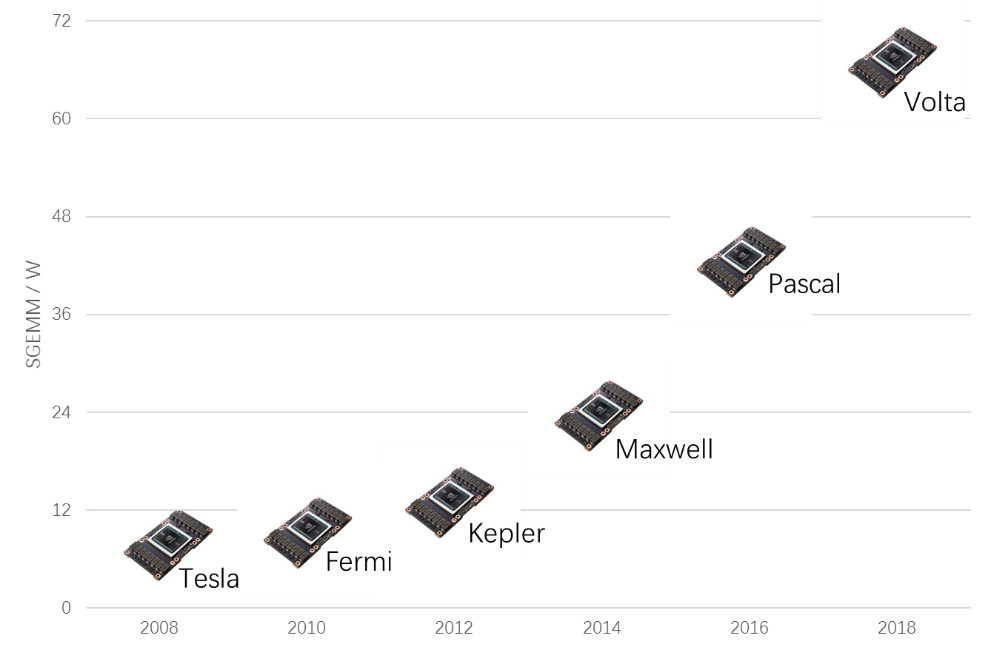
\includegraphics[width=0.40\textwidth]{nvidia_roadmap}
	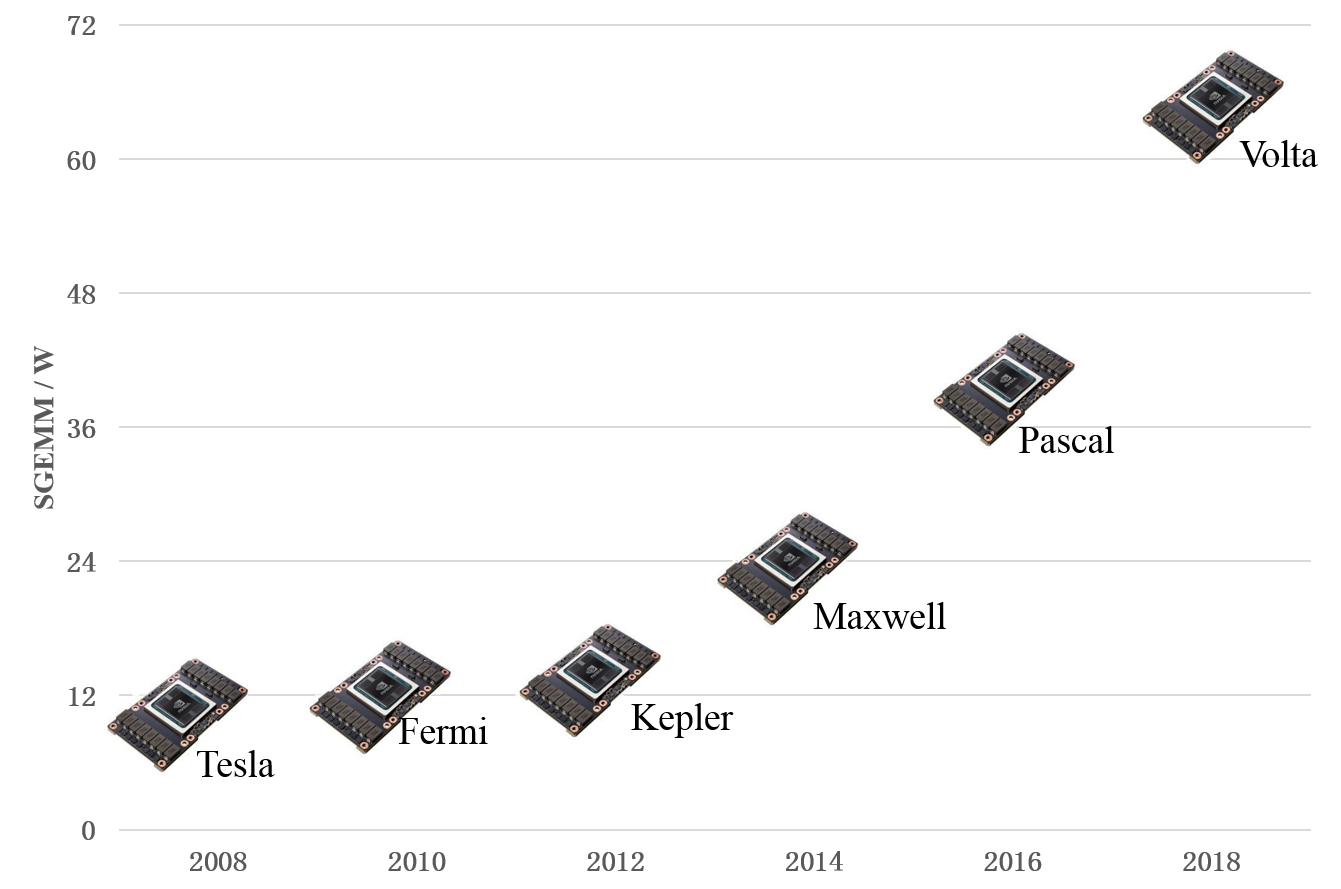
\includegraphics[width=0.80\textwidth]{nvidia_gpu_roadmap}
	\bicaption{NVIDIA GPU架构演进图}{NVIDIA GPU Architecture Evolution}
	\label{fig:nvidia_gpu_roadmap}
\end{figure}

AMD提出的GCN(Graphic Core Next)相较之前提出的VLIW架构是一个分水岭。AMD GPU历经了Polaris,Vega,Navi架构的演进(如图\ref{fig:amd_roadmap})。这几种系列的产品都采用了GCN架构。GCN架构具有灵活的可编程性,较好的编译工具链的支持,可极大发挥出GPU的计算能力。
\begin{figure}[!htbp]
	\centering
	%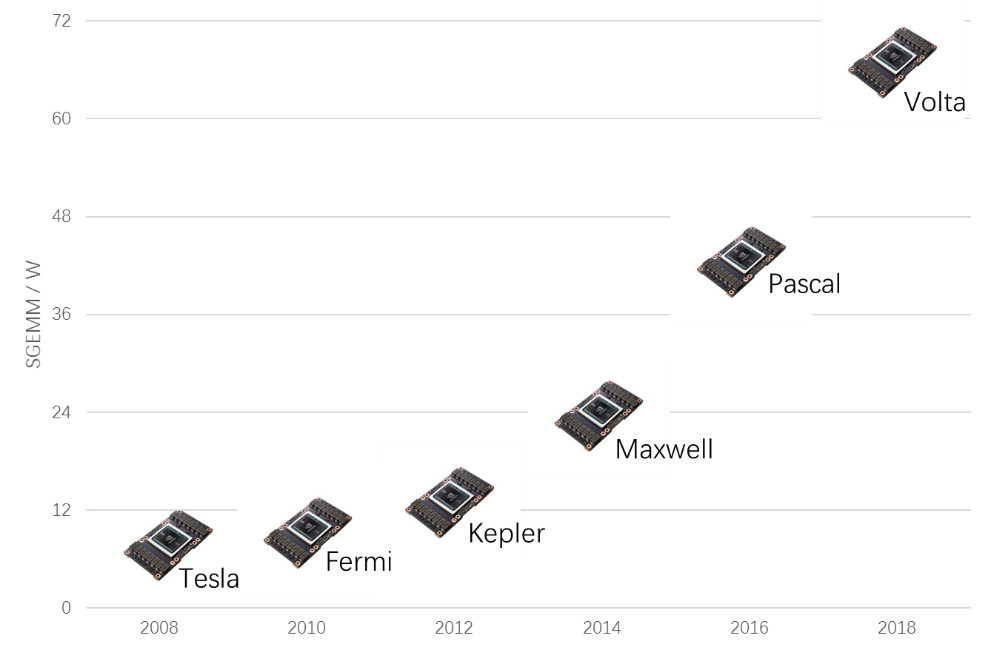
\includegraphics[width=0.40\textwidth]{nvidia_roadmap}
	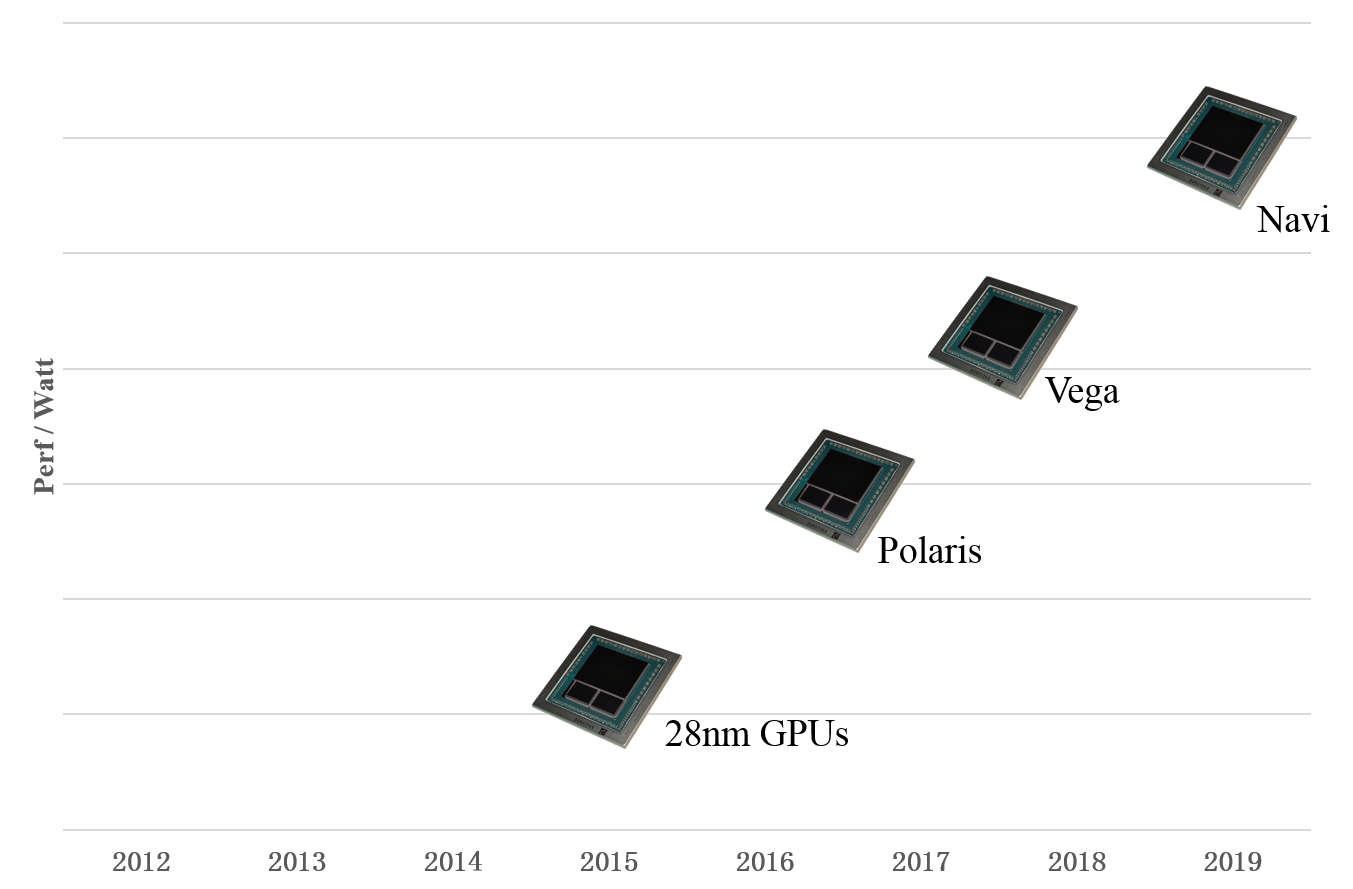
\includegraphics[width=0.80\textwidth]{amd_roadmap}
	\bicaption{AMD GPU架构演进图}{AMD GPU Architecture Evolution}
	\label{fig:amd_roadmap}
\end{figure}

\section{并行计算技术概述}
计算可分为串行计算和并行计算。为了引出并行计算的概念,我们先从串行计算开始介绍。在计算机发展的早期,程序编制人员编写的通常是串行软件。串行软件有这几个特点:(1) 将要处理的问题分解为一系列的指令,(2) 这些指令按照顺序一条一条执行,(3) 所运行的处理器只有一个核心,(4) 在同一时刻只能有一条指令在执行(如图\ref{fig:serialprogram})

\begin{figure}[!htbp]
	\centering
	%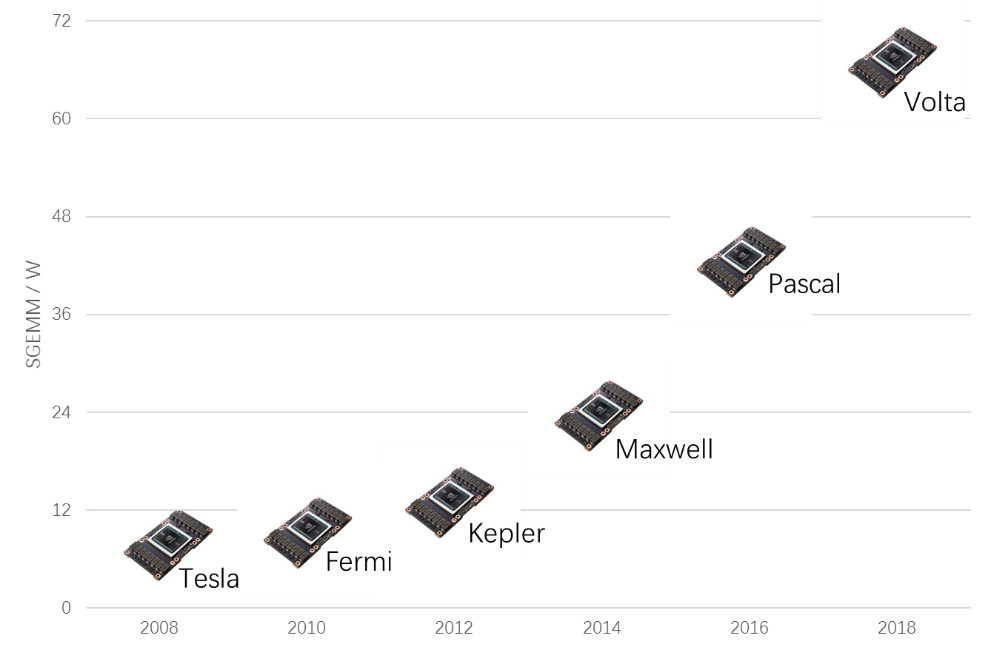
\includegraphics[width=0.40\textwidth]{nvidia_roadmap}
	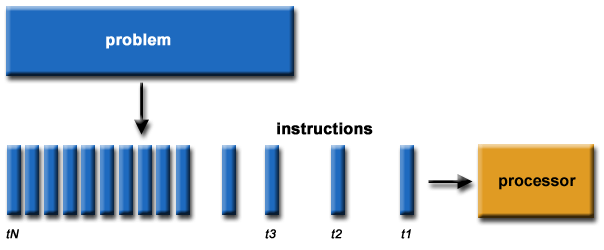
\includegraphics[width=0.80\textwidth]{serialprogram}
	\bicaption{串行程序执行示意图}{Serial program execution diagram}
	\label{fig:serialprogram}
\end{figure}

接下来引入并行计算的概念。从简单意义上来讲,并行计算是同时使用多个计算资源来解决计算问题。并行计算具有如下几个特点:(1) 将一个问题分解成可以同时求解的几个子问题,(2) 每个子问题同时在不同的处理器上计算,(3) 有一个总的控制协调机制(如图\ref{fig:parallelprogram})

\begin{figure}[!htbp]
	\centering
	%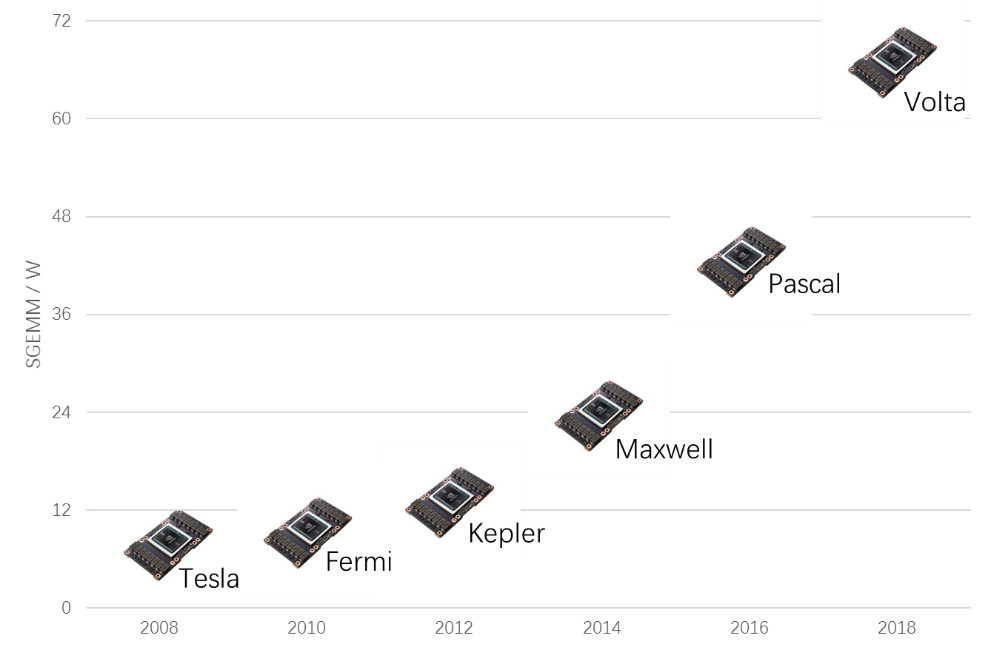
\includegraphics[width=0.40\textwidth]{nvidia_roadmap}
	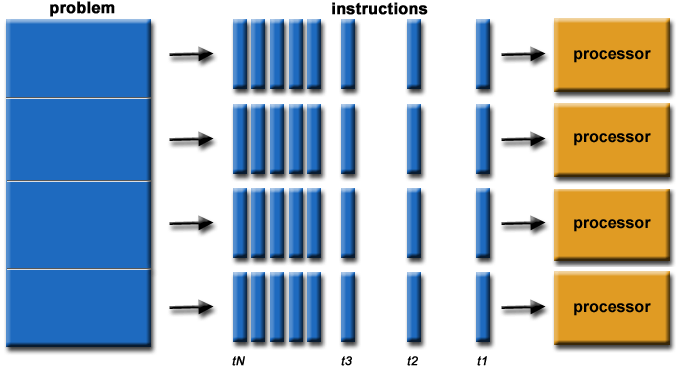
\includegraphics[width=0.80\textwidth]{parallelprogram}
	\bicaption{并行程序执行示意图}{Parallel program execution diagram}
	\label{fig:parallelprogram}
\end{figure}

并行计算的主要目标是通过提高计算资源的利用率来使得应用程序运行的更快。通常情况下,并行计算的基础设施可以是服务器机架上的一个多个处理器或者许多单独的服务器通过网络连接在一起的服务器集群。将计算任务划分成一个个子任务,Server端将每个子任务的计算请求发送到每个处理器(线程),每个处理器(线程)执行自己的子任务,最后Server端合并计算的结果。并行计算可以分为指令集并行,数据并行和任务并行。


\section{研究动机述}
矩阵乘是BLAS(Basic Liner Algebra Subprogram) Level3标准中定义的数学计算,是BLAS库的核心子程序之一。虽然BLAS规范是通用的,但是BLAS库的实现通常都针对特定硬件进行着专门的优化,使得BLAS库具有显著的性能优势。BLAS库在实现上利用特殊的浮点硬件(如向量寄存器,SIMD指令等)来提高计算速度。BLAS库的例子包括:AMD核心数学库(ACML),ATLAS,英特尔数学核心库(MKL)和OpenBLAS。ATLAS是一个可自动调优的,适用于任意硬件架构的可移植库。MKL是英特尔官方提供的针对英特尔处理器进行了专门优化的数据库。OpenBLAS是一个开源库,针对许多主流的体系结构进行了手工优化。LINPACK程序的跑分在很大程度上依赖于BLAS库中DGEMM的子程序的性能。BLAS库被广泛应用于高性能计算领域,近几年兴起的深度学习,其核心计算也依赖于BLAS库的性能。

矩阵乘的效率通常可以展示一个计算机系统实际可达的最高计算性能。通过对矩阵乘性能的调优和性能分析,可以深入理解现代多核处理器体系结构的方方面面。同时,也将提高BLAS库Level3的计算性能,从而提高基于BLAS库的应用的计算速度。

DNN(Deep Neural Network)是深度学习的一个主要方向。由于DNN的强大的表达能力,使得人们可以使用其解决各种领域里的问题。当前的DNN几乎代表了机器学习的主要发展方向。在DNN网络中,有大量的参数,使得做训练和推理的过程变得非常耗时。特别是,全连接和卷积层的矩阵乘(Matrix Multiplication)计算成为了DNN计算的瓶颈。计算机科学家和工程师们花费了很多年来研究如何提高DNN的计算效率。

在GPUs出现之后,DNN开始流行起来。因为相比于CPU,GPUs可以将矩阵乘的计算速度提升几十到几百倍。在此期间,NVIDIA开发出了专门用于DNN训练和推理的数学库cuDNN\citepns{chetlur2014cudnn},由于该库的鲁棒性和高性能,cuDNN已经成为了当前的工业标准。cuDNN中矩阵乘的实现对于各种输入尺寸,在不同的GPUs架构上都可以获得较高的性能。另外,cuDNN作为后端,已经广泛用于各种DNN框架中,例如caffe、pytorch、tensorflow和mxnet。所以,提高矩阵乘的效率,可加速DNN的训练和推理过程。


\section{本文主要贡献}
本文工作是基于AMD GPU平台,实现了面向GPU体系结构的通用矩阵乘优化,以解决当下AMD GPU矩阵乘的性能瓶颈问题,并且对AMD GPU矩阵乘进行了性能分析,为优化AMD GPU其他应用程序提供了性能分析方法。论文的主要工作如下:

% (1) 深入理解AMD GPU体系结构,比较了NVIDIA GPU和AMD GPU在架构设计上和程序执行模型上的异同。
%
% (2) 分析了NVIDIA GPU矩阵乘的效率,总结出NVIDIA GPU矩阵乘的优化手法。

 (1) 基于对NVIDIA GPU矩阵乘算法以及优化方法的理解,将该方法结合AMD新一代GPU Fiji和Vega10架构的特点,提出AMD GPU矩阵乘算法以及调优方法。

 (2) 实现了面向AMD GPU体系结构的通用矩阵乘计算,通过对AMD GPU架构的理解,进行矩阵乘的调优,提高了AMD GPU矩阵乘的效率。

 (3) 针对AMD GPU体系结构的特点,测试出浮点指令的通量,并分析了矩阵乘的性能上界。


\section{本文组织结构}
本文总共分为七章。

第一章概述了课题的研究背景。讲述GPU体系结构的发展历程以及当前主流应用对并行计算的需求,凸显本课题的研究动机和意义,并介绍了研究内容和主要贡献。

第二章介绍了技术背景和相关研究。首先对矩阵乘的几种常用算法进行描述,对每种算法的优缺点和使用场景进行简单概述。然后介绍目前已有的矩阵乘优化加速工作,分析其方法的优点以及存在的问题。

第三章对主流的多核和并行处理器体系结构的原理进行详细介绍,分析多核体系结构对程序性能的影响,为后文讲述矩阵乘算法在AMD GPU平台上的实现进行铺垫。

第四章介绍了GPU体系结构的特点,GPU程序的组织和执行模式。包括了GPU的内存层次结构,GPU的计算单元的组织方式,GPU的硬件计算单元如何与软件线程关联起来,GPU的编程模型,程序的执行模式。其中核心的概念是GPU的SIMD(或SIMT)执行方式。NVIDIA和AMD GPU在设计上都采用这种执行方式。

第五章讲述了矩阵乘GPU实现的算法和具体实现步骤。描述了矩阵乘外积法的执行过程,并分析了外积法相比于內积法的优势。通过三个步骤讲述了外积法矩阵乘计算过程中,数据的搬运和计算的执行过程。为下一章节讲述矩阵乘调优过程做铺垫。

第六章以AMD Fiji和Vega10 GPU为实验平台,进行了AMD GPU矩阵乘算法的设计和调优。进行矩阵乘性能测试,分析AMD GPU矩阵乘性能上界。

第七章对全文进行总结,并提出未来可能的研究方向。



